\documentclass[tikz,border=5pt]{standalone}
\usepackage{fontspec}
\setmainfont{Times New Roman}
\usepackage{unicode-math}
\setmathfont{Cambria Math}
\usetikzlibrary{shapes.geometric,shapes.misc,positioning,fit,backgrounds,arrows.meta,calc}

\begin{document}
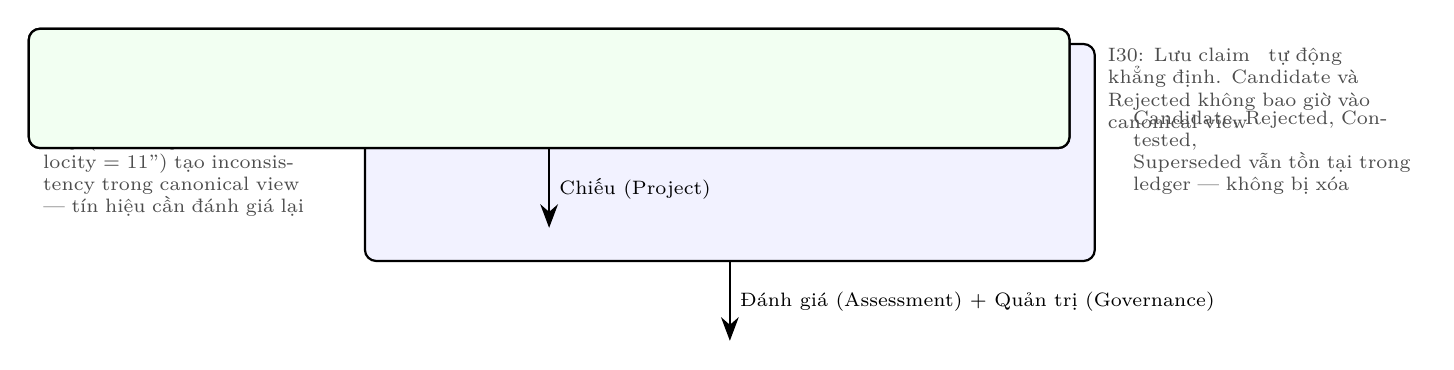
\begin{tikzpicture}[
    chip/.style={rectangle, draw, rounded corners, minimum width=3.2cm, minimum height=0.55cm, font=\scriptsize},
    fitbox/.style={rectangle, draw, thick, rounded corners, inner sep=8pt},
    arrow/.style={-{Stealth[length=3mm]}, thick},
    note/.style={font=\scriptsize, text=gray!60!black, align=left, text width=3.6cm},
    label/.style={font=\small\bfseries},
]

% ---- Claim Ledger: chips in a grid, fit box around them ----
\node[chip, fill=green!20] (c1) {ex:claim\_roc\_A :: Accepted};
\node[chip, fill=gray!15, right=0.4cm of c1] (c5) {ex:claim\_speed :: Rejected};
\node[chip, fill=yellow!20, below=0.25cm of c1] (c2) {ex:claim\_roc\_rel :: Contested};
\node[chip, fill=red!15, right=0.4cm of c2] (c3) {ex:claim\_pop\_old :: Superseded};
\node[chip, fill=blue!10, below=0.25cm of c2] (c4) {ex:claim\_pop\_est :: Candidate};

\node[fitbox, fill=blue!5, fit=(c1)(c2)(c3)(c4)(c5), label={[label]above:Claim Ledger (toàn bộ phát biểu)}] (ledger) {};

\node[note, right=0.35cm of ledger.east] {Candidate, Rejected, Contested, \\ Superseded vẫn tồn tại trong ledger — không bị xóa};
\node[note, left=0.35cm of ledger.west] {I31: Hai claim Accepted cùng valid time, cùng property ("velocity = 10" vs "velocity = 11") tạo inconsistency trong canonical view — tín hiệu cần đánh giá lại};

% ---- Assessment / Governance step ----
\draw[arrow] (ledger.south) -- node[right, font=\scriptsize] {Đánh giá (Assessment) + Quản trị (Governance)} ++(0,-1.0);

% ---- Projection Policy: rules text in a fit box ----
\node[align=left, font=\scriptsize, text width=12.5cm, inner sep=2pt] (rules) {
  • Status = Accepted (loại trừ Candidate, Rejected, Contested, Superseded)\\
  • Valid time chứa thời điểm hiện tại\\
  • Nếu nhiều claim cùng thỏa mãn: ưu tiên evidence mạnh nhất
};
\node[fitbox, fill=orange!5, fit=(rules), label={[label]above:Chính sách chiếu (Projection Policy)}] (policy) {};

% ---- Project step ----
\draw[arrow] (policy.south) -- node[right, font=\scriptsize] {Chiếu (Project)} ++(0,-1.0);

% ---- Canonical Knowledge View: content text in a fit box ----
\node[align=left, font=\scriptsize, text width=12.5cm, inner sep=2pt] (proj) {
  • `ex:Hanoi ex:capitalOf ex:Vietnam` (từ claim\_hanoi\_capital, Accepted)\\
  • `ex:rateOfChange\_1 ex:hasOperation ex:derivativeOperation\_1` (từ claim\_roc\_A, Accepted)\\
  • Được coi là "đúng" cho truy vấn mặc định của hệ thống
};
\node[fitbox, fill=green!5, fit=(proj), label={[label]above:Canonical Knowledge View (tầng nhìn chuẩn hóa)}] (view) {};

\node[note, right=0.35cm of view.east] {I30: Lưu claim ≠ tự động khẳng định. Candidate và Rejected không bao giờ vào canonical view};

\end{tikzpicture}
\end{document}